\chapter{Dezvoltări ulterioare și posibile limitări}
\label{chap:next}
Ca scopuri pentru dezvoltarea ulterioară a proiectului pot menționa testarea și implementarea ideilor din \autoref{chap:extra}, dar și rezolvarea problemelor cărora nu le-am găsit încă o soluție.
\section{Problema numărării vehiculelor pe străzi cu mai multe benzi de circulație}
Una dintre aceste probleme este activarea senzorilor la momentul trecerii unui vehicul pe cealaltă banda de circulație. În exemplul din \figref{fig:dezv}, aplicat modelului din \autoref{hw}, vehiculul ar incrementa counter-ul corespunzător următoarelor felinare de 2 ori cu o singură trecere.
 
\begin{figure}[!ht]
    \begin{center}
    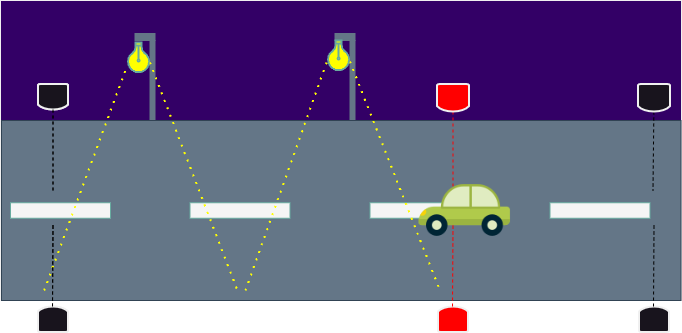
\includegraphics[width=0.6\linewidth,keepaspectratio]{pics/dezv.png}
    \end{center}
    \caption{Activare simultană a 2 senzori}
    \label{fig:dezv}
\end{figure}

 Data viitoare când acesta se află în întregime pe o singură bandă, el va decrementa counter-ul din urmă doar cu 1, iar consecința va fi o desincronizare dintre valorile din counter și numărul real de vehicule de pe stradă (rezultat asemănător și în cazul situației din \autoref{rev}).  Nici micșorarea razei de detecție a senzorilor nu rezolvă această problemă, deoarece sunt create situații în care un vehicul poate trece prin mijlocul drumului complet neobservat, cauzând aceeași desincronizare menționată anterior. Aici m-am gândit la suplimentarea cu metode de măsurat a distanței de la senzori, prin adăugarea, de exemplu, a senzorilor ultrasonici menționați în \autoref{collect}. Un dezavantaj este faptul că nu am lucrat cu astfel de senzori, deci nu cunosc toate limitările ce pot fi întâlnite în practică. 

Problema numărării vehiculelor apare și în cazul străzilor cu mai mult de 2 benzi pe același sens de circulație, deoarece 2 astfel de senzori plasați pe părți opuse ale străzii nu pot diferenția între 2 sau mai multe automobile care trec în același timp. 


\section{Problema calculării vitezei pe străzi cu mai multe benzi de circulație}


Pe orice stradă pe care este posibilă depășirea vehiculelor, calculul vitezei devine greu de realizat, deoarece acesta se realizează cu presupunerea că primul vehicul care intră într-o porțiune de drum va fi și primul care iese din ea. Aceasta este, în opinia mea, cea mai mare limitare a sistemului în starea sa actuală. În schimb, chiar și în cazul eliminării componentei de măsurat viteza, performantele obținute ar fi, în continuare, satisfăcătoare din punct de vedere al consumului de energie electrică. Pentru studiul din \cite{7513906}, unde consumul pe durata unei luni a scăzut cu 40\%, felinarele funcționează la intensitate maximă la detecția unui vehicul, indiferent de viteza acestuia.

 \section{Caz particular pietoni}

Detecția pietonilor poate fi considerată un caz particular de stradă cu mai multe benzi de circulație.  Principalele diferențe sunt dificultatea în a determina comportamentul acestora și faptul că viteza lor nu este la fel de relevantă ca cea a vehiculelor. Senzorii pentru prezență destinați detectării pietonilor trebuie să fie separați de cei pentru automobile, pentru a nu influența măsurarea vitezei acestora, ca în \figref{fig:ped}. 
 \begin{figure}[!ht]
    \begin{center}
    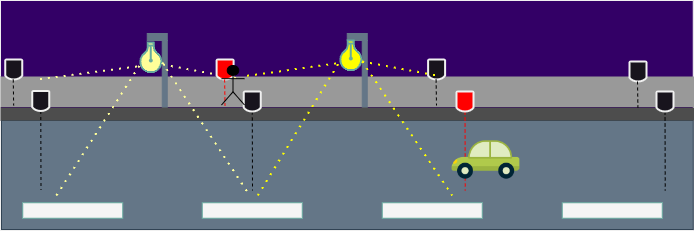
\includegraphics[width=0.8\linewidth,keepaspectratio]{pics/ped.png}
    \end{center}
    \caption{Sugestie sistem pentru detectarea pietonilor}
    \label{fig:ped}
\end{figure}

Direcția deplasării pietonilor nu poate fi prezisă cu certitudine. Aceștia se pot și opri sau părăsi drumul, de exemplu pentru a intra într-o clădire. De aceea, sunt de părere că trecerea pietonilor nu ar trebui să influențeze counter-ul ce determină funcționarea felinarelor, ci doar să aprindă cele două sau mai multe felinare din jurul senzorului activat, la intensitate medie, în cazul în care acestea nu erau deja aprinse. Pentru această metodă, este necesară adăugarea unui timer(\ref{timer}) , care să determine stingerea felinarelor la trecerea unei perioade de timp prestabilite.

\section{Utilizare timere} \label{timer}

Arduino IDE permite folosirea unor funcții specializate pentru realizarea operațiilor cu momente de timp, prin adăugarea de biblioteci ce se bazează pe funcțiile millis() sau micros(). Atât folosirea unor timere ca unică metodă de control a stingerii felinarelor, cât și îmbinarea unui astfel de element cu sistemul realizat, poate oferi performanțe mai bune în cazurile limită. Aceasta pare a fi chiar obligatorie pentru orice fel de astfel de sistem care are ca scop și detectarea pietonilor. În metoda mea de implementare am preferat să nu adaug timere, pentru a evidenția cât mai mult răspunsurile sistemului la stimuli externi, specifice unui sistem în timp real. 

Un exemplu de posibilă îmbunătățire adusă de adăugarea unui timer este decrementarea automată a counter-ului $\mathbf{c}$ pentru o anumită porțiune de drum, la trecerea unei perioade de timp prestabilită de la ultima dată când a intrat un vehicul în ea. Aceasta ar duce la stingerea felinarului în cazul în care un vehicul se oprește între 2 senzori, sau dacă acesta, din posibile erori hardware, nu este detectat de senzorul de la ieșirea din porțiunea respectivă. 
